\documentclass[border=8pt]{standalone}
\usepackage[T1]{fontenc}
\usepackage{xcolor}
\usepackage{amsmath}
\usepackage{siunitx}
\usepackage{tikz}
\usetikzlibrary{arrows.meta,positioning,shapes.geometric,calc,fit,backgrounds}
\usepackage[siunitx,american]{circuitikz}
\usepackage{mathptmx}
\definecolor{ink}{HTML}{14202B}
\definecolor{slate}{HTML}{24394B}
\definecolor{amber}{HTML}{C9781E}
\definecolor{amberlight}{HTML}{FBEBD3}
\definecolor{teal}{HTML}{3E7F8C}
\definecolor{paper}{HTML}{F6F3EC}
\definecolor{muted}{HTML}{5E6974}

\newcommand{\code}[1]{\texttt{#1}}
\tikzset{
  blk/.style={draw=slate,rounded corners=3pt,fill=white,align=center,font=\small,minimum height=0.9cm,text width=3.3cm},
  hub/.style={draw=amber,line width=1.1pt,rounded corners=4pt,fill=amberlight,align=center,font=\small},
  arr/.style={-{Stealth[length=2.2mm]},draw=slate,line width=0.7pt},
  stp/.style={draw=slate,rounded corners=3pt,fill=white,align=center,font=\small,minimum height=1.1cm,text width=4.2cm},
}

\begin{document}
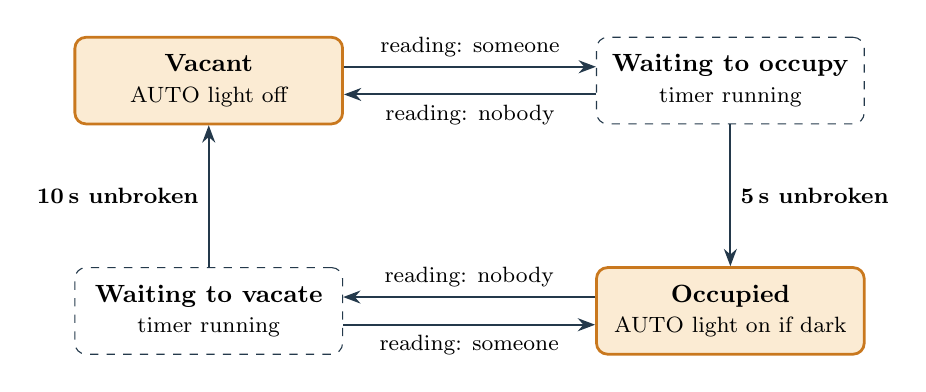
\begin{tikzpicture}[node distance=1.2cm and 3.2cm,
  st/.style={draw=slate,rounded corners=4pt,align=center,font=\small,minimum width=3.4cm,minimum height=1.1cm},
  stable/.style={st,draw=amber,line width=1pt,fill=amberlight},
  wait/.style={st,dashed}]
\node[stable] (v) {\textbf{Vacant}\\\footnotesize AUTO light off};
\node[wait,right=of v] (wo) {\textbf{Waiting to occupy}\\\footnotesize timer running};
\node[stable,below=1.8cm of wo] (o) {\textbf{Occupied}\\\footnotesize AUTO light on if dark};
\node[wait,below=1.8cm of v] (wv) {\textbf{Waiting to vacate}\\\footnotesize timer running};
\draw[arr] ([yshift=5pt]v.east) -- node[above,font=\footnotesize]{reading: someone} ([yshift=5pt]wo.west);
\draw[arr] ([yshift=-5pt]wo.west) -- node[below,font=\footnotesize]{reading: nobody} ([yshift=-5pt]v.east);
\draw[arr] (wo) -- node[right,font=\footnotesize\bfseries]{5\,s unbroken} (o);
\draw[arr] ([yshift=5pt]o.west) -- node[above,font=\footnotesize]{reading: nobody} ([yshift=5pt]wv.east);
\draw[arr] ([yshift=-5pt]wv.east) -- node[below,font=\footnotesize]{reading: someone} ([yshift=-5pt]o.west);
\draw[arr] (wv) -- node[left,font=\footnotesize\bfseries]{10\,s unbroken} (v);
\end{tikzpicture}
\end{document}
